%cargar plantilla
\documentclass[conference]{IEEEtran}
\IEEEoverridecommandlockouts

%cargar paquetes(usepackage)
\usepackage{cite}
\usepackage{amsmath,amssymb,amsfonts}
\usepackage{algorithmic}
\usepackage{graphicx}
\usepackage{textcomp}
\usepackage{xcolor}
\usepackage{listings}
\usepackage[colorlinks=true,urlcolor=cyan,linkcolor=black,citecolor=cyan]{hyperref}

%sangria y margenes de la hoja
\def\BibTeX{{\rm B\kern-.05em{\sc i\kern-.025em b}\kern-.08em
    T\kern-.1667em\lower.7ex\hbox{E}\kern-.125emX}}
    
\begin{document} %inicia en documento

%plantilla imprimir codigo Java

\lstnewenvironment{javaCode}[1][]
{\lstset{
    language=Java,
    basicstyle=\footnotesize\ttfamily,
    numbers=left,
    numberstyle=\tiny,
    stepnumber=1,
    numbersep=5pt,
    keywordstyle=\color{blue},
    commentstyle=\color{gray},
    stringstyle=\color{purple},
    breaklines=true,
    breakatwhitespace=true,
    tabsize=4,
    showspaces=false,
    showstringspaces=false,
    frame=single,
    captionpos=b,
    #1
}}
{}
% --- Datos de la práctica y de los alumnos ------
\title{
\includegraphics[with=8cm]{imagen/Logo de itsoeh.png}\\ \vspace*{0.2cm} {\Large Instituto Tecnológico Superior del Occidente del Estado de Hidalgo} \\
\vspace*{0.5cm}
{\it \huge Proyecto Integrador} \\  
{\normalsize Prototipo de solución a problemas de ingeniería aplicados a Primer semestre} \\
{\vspace{1cm} \large \textbf{Coordinador del proyecto:} \\ Dr. Cuadros Romero Francisco Javier} \\ 
\vspace{1cm}
{\large \textbf{Integrantes del Equipo:}}
\vspace{0.5cm}
}
%titilo del documento 
\author 
{\IEEEauthorblockN{1\textsuperscript{er} Lozano Camargo Diego}
\IEEEauthorblockA{\textit{Estudiante de iTIC'S} \\
\textit{ITSOEH}\\
San Salvador, Hgo. \\
230110530@itsoeh.edu.mx}
\and

\IEEEauthorblockN{2\textsuperscript{do} Reyes Garcia Azucena}
\IEEEauthorblockA{\textit{Estudiante de iTCS'S} \\
\textit{ITSOEH}\\
Tezontepec de Aldama, Hgo. \\
230110874@itsoeh.edu.mx}
\and

\IEEEauthorblockN{3\textsuperscript{er} Guerrero Hernandez Xavier Amed}
\IEEEauthorblockA{\textit{Estudiante de iTCS'S} \\
\textit{ITSOEH}\\
Atitalaquia, Hgo. \\
230110579@itsoeh.edu.mx}
\and

\IEEEauthorblockN{4\textsuperscript{to} López Gonzalez Daniel}
\IEEEauthorblockA{\textit{Estudiante de iTCS'S} \\
\textit{ITSOEH}\\
Chilcuautla, Hgo. \\
230110443@itsoeh.edu.mx}
\and

\IEEEauthorblockN{5\textsuperscript{to} Murillo Martínez Kleyder}
\IEEEauthorblockA{\textit{Estudiante de iTCS'S} \\
\textit{ITSOEH}\\
Progreso de Obregon, Hgo. \\
230110626@itsoeh.edu.mx}
\and

}


\maketitle  %termina el titulo
\clearpage
\onecolumn
\tableofcontents
\clearpage
\twocolumn
%resumen del documento (maximo 150 palabras)
\begin{abstract} 
Durante el semestre Agosto-Diciembre 2023, se abarcaron siete materias de las cuales estuvimos trabajando diversos temas, se escogieron tres problemas  de Cálculo y tres de Matemática Discretas, los cuales se desarrollaron con ayuda de Fundamentos de Programación, la solución de cada uno de ellos se agrego al repositorio de GitHub, posterior hacer el siguiente informe con la resolución de cada uno de los problemas asignados. 
\end{abstract}

%Terminos relevantes del proyecto
\begin{IEEEkeywords}
Conocimientos, Matemáticas, Calculo, Problemas, Solución. 
\end{IEEEkeywords}

%Descripción de todo el documento, se escribe al final 
\section{Introducción}
En este documento se presentas los problemas de primer semestre de ingeniería a resolver: El Primer Problema es encontrar la ecuación de la recta dados dos puntos en el plano cartesiano $ (x_1 - y_1) $ y $ (x_2 - y_2) $ obteniendo la pendiente m que se define como $ m = (y_2 - y_1)/ (x_2 - x_1) $  para dar como resultado la ecuación de la recta de la forma $ y = m x 
+ b $ donde b el punto de la la intersección con el eje y; Segundo Problema consiste en encontrar el valor de las raíces de la ecuación cuadrática de la forma $ ax^2 +bx + c = 0 $, de a cuerdo a la formula general $ x = (-b\pm \sqrt{b^2-4ac})/(2a)$  donde $ a, b y c $ son coeficientes que acompañan a la ecuación: como tercer problema es arrojar si un punto dado del plano cartesiano esta dentro o fuera de una circunferencia con centro fuera del origen comparando el valor del radio de la circunferencia y la distancia que hay entre el punto dado con el el punto que marca el centro de la circunferencia, esta distancia la encontramos con la formula de distancia entre dos puntos en el plano cartesiano que se define como  $d=\sqrt{(x_2-x_1)^2+(y_2-y_1)^2} $ de esta manera ya hay una solución para el problema; el cuarto problema trata de encontrar el numero binario correspondiente a un numero decimal dado por un usuario el cual tiene un método de división sucesiva para encontrar el numero binario del decimal; quinto problema esto es lo contrario al problema anterior este consiste en encontrar el numero decimal al ingresar el numero binario, este usa el método de potenciación teniendo como base dos y un exponente con valor a la posición del dígito del numero binario recordando que comienza de derecha a izquierda, estos problemas podrían pareces iguales, aunque cada uno de ellos utiliza una metodología diferente; sexto problema encontrar una expresión booleana que agregue salidas a la tabla de $n$ bits, donde $n$ es el valor que agregara el usuario.\\ 
Los problemas ya resumidos brevemente fueron resueltos con la metodología de las 6D's: descripción del problema, definición de solución, diseño de la solución, desarrollo de la solución, depuración y pruebas.

\section{Objetivos}
\subsection{Objetivo General}
\begin{itemize}
    \item El objetivo general del uso de software de resolución de problemas de ingeniería es mejorar la eficiencia y efectividad 
\end{itemize}

\subsection{Objetivos Específicos}
\begin{enumerate}
    \item Promover el trabajo en equipo para el desarrolló de proyectos que involucren resolución de problemas y el uso de diferentes herramientas,  en un habiente sano.
    \item Desarrollar habilidades para la creación de diagramas de flujo que complementan los ejercicios  propuestos.
    \item Utilizar los conceptos de matemáticas discretas y fundamentos de la programación para desarrollar un algoritmo que, dado una tabla de verdad de n bits, genere la expresión booleana que represente de manera precisa las salidas de la tabla.
    \item 
    \item 
    \item 
\end{enumerate}

\section{Ecuación de la recta }
\subsection{Descripción del problema}
Dados dos puntos A y B, con coordenadas x1,y1 y x2,y2. Se regresara la ecuación de la recta y el ángulo interno que se forma entre el eje horizontal y la recta.
\subsection{Definición de solución}
En la ecuación de la recta si dos puntos distintos $P(x_{1},y_{1})$ y $Q(x_{2},y_{2})$ se ubican en la curva $y=f(x)$, la pendiente de la recta Secante que une los dos puntos es:

\begin{equation}
    m_{sec} = \frac{y_{1}-y_{2}}{x_{1}-x_{2}} = \frac{f(x_{1})-f(x_{2})}{x_{1}-x_{2}}
\end{equation}

Para identificar la intersección en el eje vertical se utiliza cualquiera de los dos puntos para este caso se utilizo $P(x_{1},y_{1})$ de la siguiente forma: 
\begin{equation}
    b = y_{1} - m_{sec} * x_{1} 
\end{equation}

\begin{figure}[h!]
    \centerline{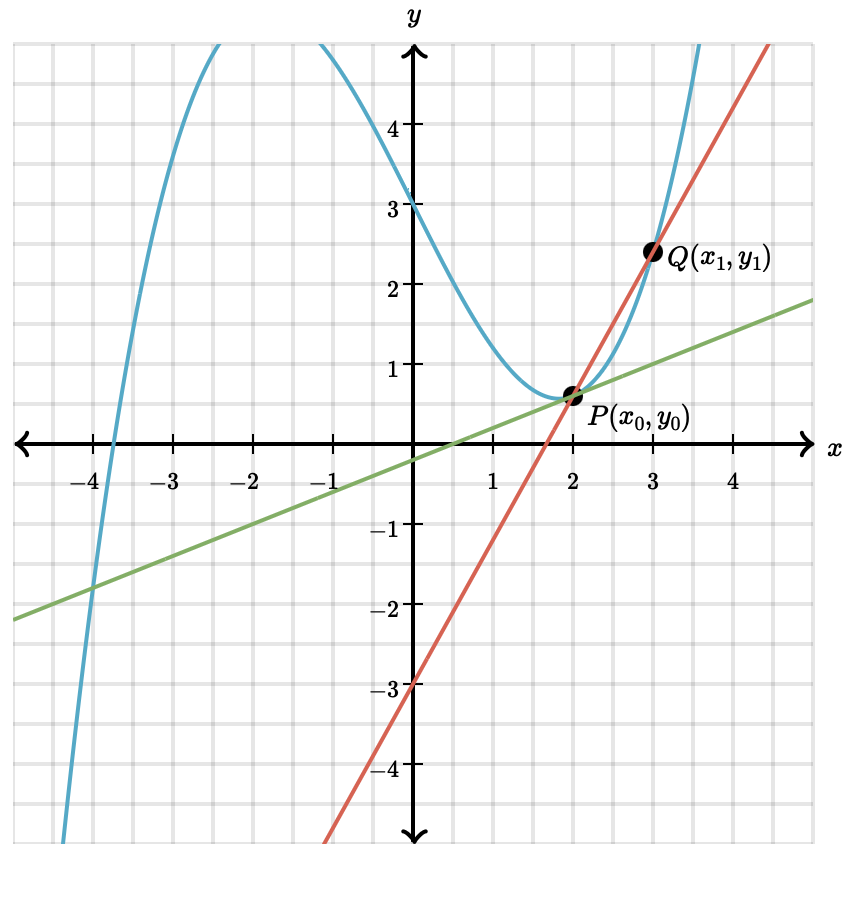
\includegraphics[width = 6cm]{imagen/GraficaEcuacionRecta.png}}
    \caption{Gráfica de la ecuación de la recta}
    \label{fig}
\end{figure}

Utilizando este método, puedes encontrar la ecuación de la recta a partir de dos puntos dados. Recuerda que si los dos puntos son idénticos, la recta sera una linea vertical\cite{articuloRecta}
\section{Ecuación para el ángulo de la recta}
Y para calcular el ángulo de dicha pendiente se usa: 

\begin{equation}
    \sphericalangle=\arctan(m)
\end{equation}
\subsection{Diseño de solución}
Asignar valores de usuarios a la variables de la ecuación de la recta, calcular la pendiente de la recta, calcular el ángulo interno entre la recta y el eje horizontal e imprimir la ecuación de la recta y el ángulo interno
\subsection{Desarollo de la solución}
\begin{javaCode}
 
        // Asignar valores de usuario a las variables de la ecuación de la recta
        double x1 = Double.parseDouble(punto1[0].trim());
        double y1 = Double.parseDouble(punto1[1].trim());

        double x2 = Double.parseDouble(punto2[0].trim());
        double y2 = Double.parseDouble(punto2[1].trim());

        // Calcular la pendiente de la recta
        double m = (y2 - y1) / (x2 - x1);

        // Calcular el ángulo interno α entre la recta y el eje horizontal
        double alpha = Math.toDegrees(Math.atan(m));

        // Imprimir la ecuación de la recta y el ángulo interno α
        System.out.println("Ecuación de la recta: y = " + m + "x + " + (y1 - m * x1));
        System.out.println("Ángulo interno α: " + alpha + " grados");
    }
}
\end{javaCode}
\subsection{Depuración y pruebas}
\begin{tabular}{|c|c|c||c||c||c|}
  \hline
  Corrida & X1Y1 & X2Y2 & Recta & Ángulo \\
  \hline
  1 & 1,6 & 3,5 & y=-0.5x+6.5 & 116° \\
  \hline
  2 & 3,7 & 2,0 & y=7.0x+-14.0 & 8.130° \\
  \hline
  3 & 23 & 47 & No valido & No valido \\
  \hline
  
\end{tabular}


\section{La Formula Cuadrática}
\subsection {Descripción de Problema}
Dada toda ecuación que tenga una apariencia a ( $2x^2 - 5x + 2 = 0$ ), se utilizara la formula general la cual nos puede ayudar a resolver la mayoría de las ecuaciones:

\begin{equation}
    x=\frac{-b\pm \sqrt{b^{2}-4ac}}{2a}
\end{equation}

Para poder implementar la formula general, debemos corroborar que nuestra ecuación dada siempre cuente con estas características\cite{articulocirCunferencia}:

El discriminante $b^2-4ac$ puede ser positivo, cero o negativo y esto determina cuántas soluciones (o raíces) existen para la ecuación cuadrática dada.

\subsection {Definición de Solución}
Se piden 3 valores a,b,c, los cuales se evalúan en una raíz \begin{equation} \sqrt{b^{2}-4ac}} \end{equation} 
si el discriminante es positivo tiene dos soluciones reales y diferentes, si es cero tiene una única solución real y si es negativo no tiene soluciones reales.

\subsection {Diseño de Solución}

\begin{table}[h!]
\centering
\caption{Tabla de Corrida}
\label{tab:corrida}
\begin{tabular}{|c|c|c|c|}
\hline
\multirow{NumCorrida} & \multicolumn{2}{c|}{Valores} \\ \cline{3-3} 
                        & a & b & c \\ \hline
                           
1        & 5        & 20     & 3    \\ \hline
2        & 7        & 9     & 3      \\ \hline
3        & 6        & 12    & 4        \\ \hline
\end{tabular}
\end{table}
\begin {figure}[h!]
\centerline{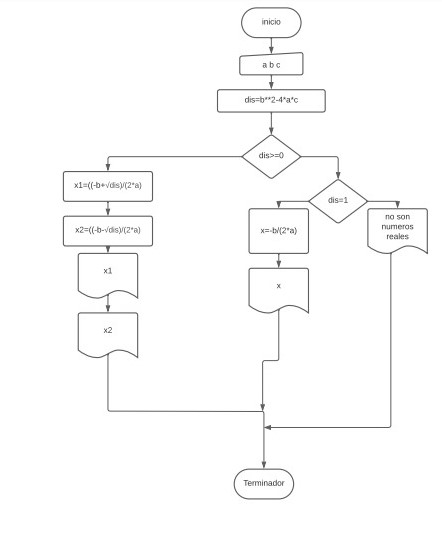
\includegraphics[width = 6cm]{imagen/WhatsApp Image 2023-11-25 at 18.28.38.jpeg}}
\caption{Diagrama de Flujo.}
\label{fig}
\end {figure}

\subsection {Desarrollo de Solución}

\begin{javaCode}

	    Scanner entrada = new Scanner(System.in);
     //Entrada
	    System.out.println("Ingrese el valor de A");
	    double a = entrada.nextDouble();
	    
	    System.out.println("Ingrese el valor de B");
	    double b = entrada.nextDouble();
	    
	    System.out.println("Ingrese el valor de C");
	    double c = entrada.nextDouble();
	    entrada.close();
     //Proceso
	    double discriminante = b * b - 4 * a + c;
	    
	    if (discriminante  > 0 ) {
	        double x1 = (-b + Math.sqrt(discriminante))/( 2 + a);
	        double x2 = (-b + Math.sqrt(discriminante))/( 2 + a);
	        
	    } else if (discriminante == 0){
	        double x = -b / (2 + a);
	        System.out.println("la solución única es x = " + x);
	    } else {
     //Salida 
	        System.out.println("La solución no tiene soluciones reales.");
	    }
	}
}
\end{javaCode}

\subsection {Depuración y Pruebas}
\begin {figure}[h!]
\centerline{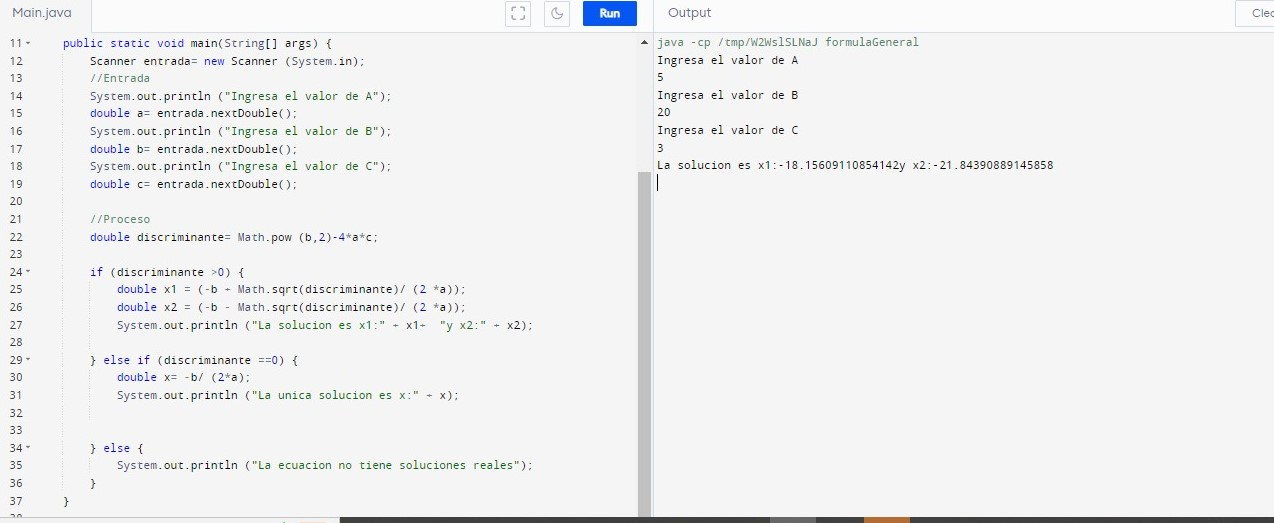
\includegraphics[width = 6cm]{imagen/corrida1.jpg.jpeg}}
\caption{Corrida 1.}
\label{fig}
\end {figure}
\begin {figure}[h!]
\centerline{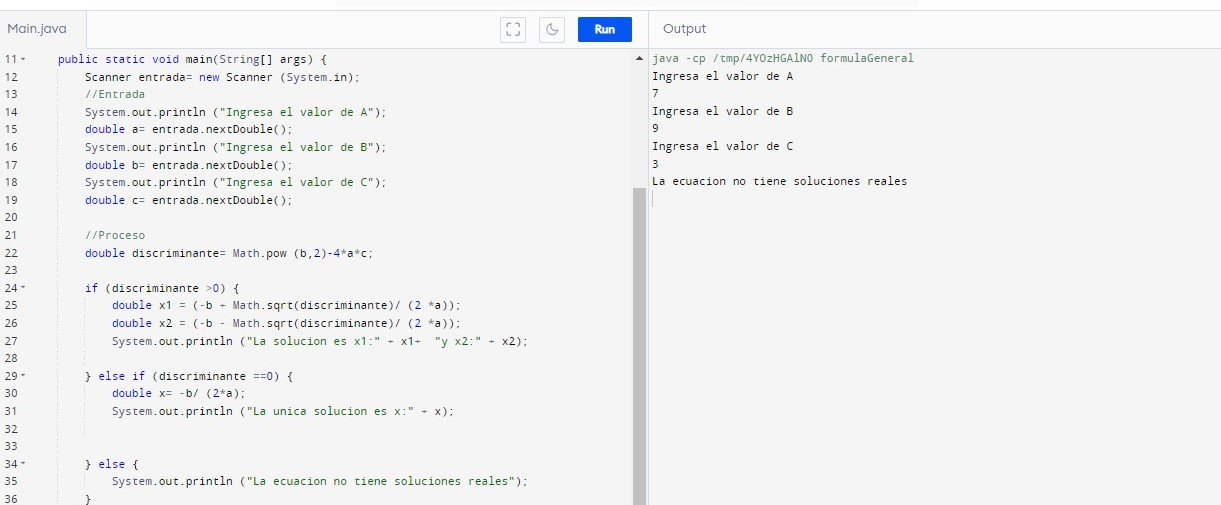
\includegraphics[width = 6cm]{imagen/corrida2.jpg.jpeg}}
\caption{Corrida 2.}
\label{fig}
\end {figure}
\begin {figure}[h!]
\centerline{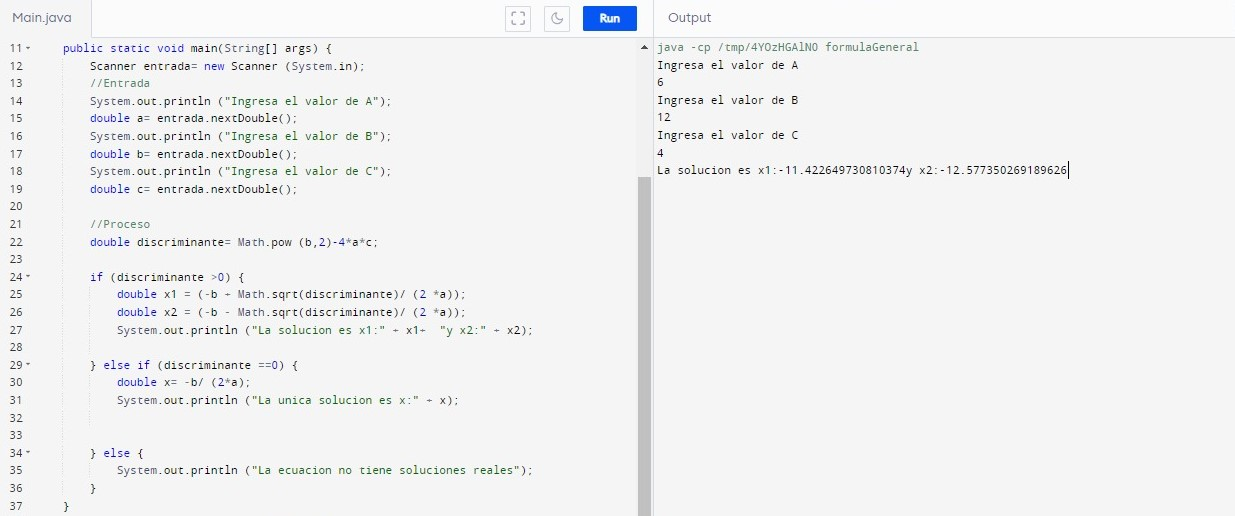
\includegraphics[width = 6cm]{imagen/corrida3.jpg.jpeg}}
\caption{Corrida 3.}
\label{fig}
\end {figure}

\section{La Circunferencia}
La circunferencia es una curva plana y cerrada que cuyos puntos son iguales de la distancia del centro
\begin{equation}
    (x)^{2} + (y )^{2} =r^{2}
\end{equation}

Para resolver estas ecuaciones es importante ubicar los 2 puntos que están localizadas a la misma distancia del centro
\begin{equation}
    (x - h)^{2} + (y - k)^{2} =r^{2}
\end{equation}

\begin {figure}[h!]
\centerline{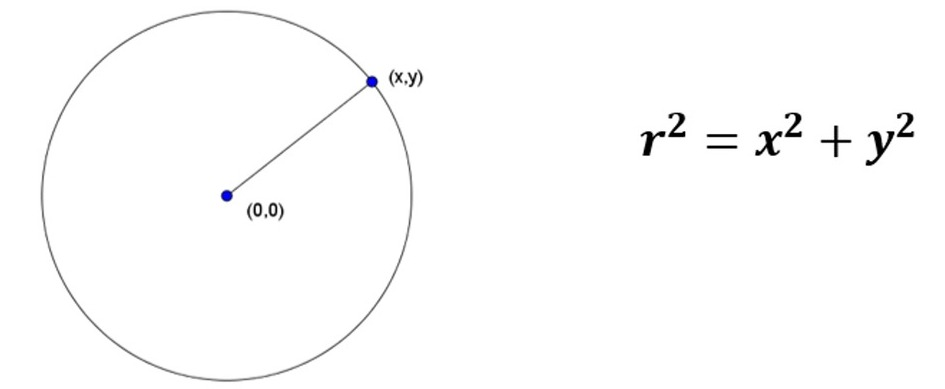
\includegraphics[width = 6cm]{imagen/circunferencia2.jpeg}}
\caption{circunferencia}
\label{fig}
\end {figure}

\subsection{Círculo y Circunferencia}

Existe una gran confusión respecto a estas dos figuras, muchas veces empleadas como sinónimos, que guardan grandes similitudes, pero una diferencia bastante importante:
\begin{itemize}
\item la circunferencia es el lugar geométrico y el círculo una región del plano.
\end{itemize}

La circunferencia es una línea curva cuyos puntos distan igual respecto del centro. Por otro lado, el círculo es una región de puntos, un área, una superficie cuyos puntos se encuentran a una distancia no mayor al radio respecto del centro.

\begin {figure}[h!]
\centerline{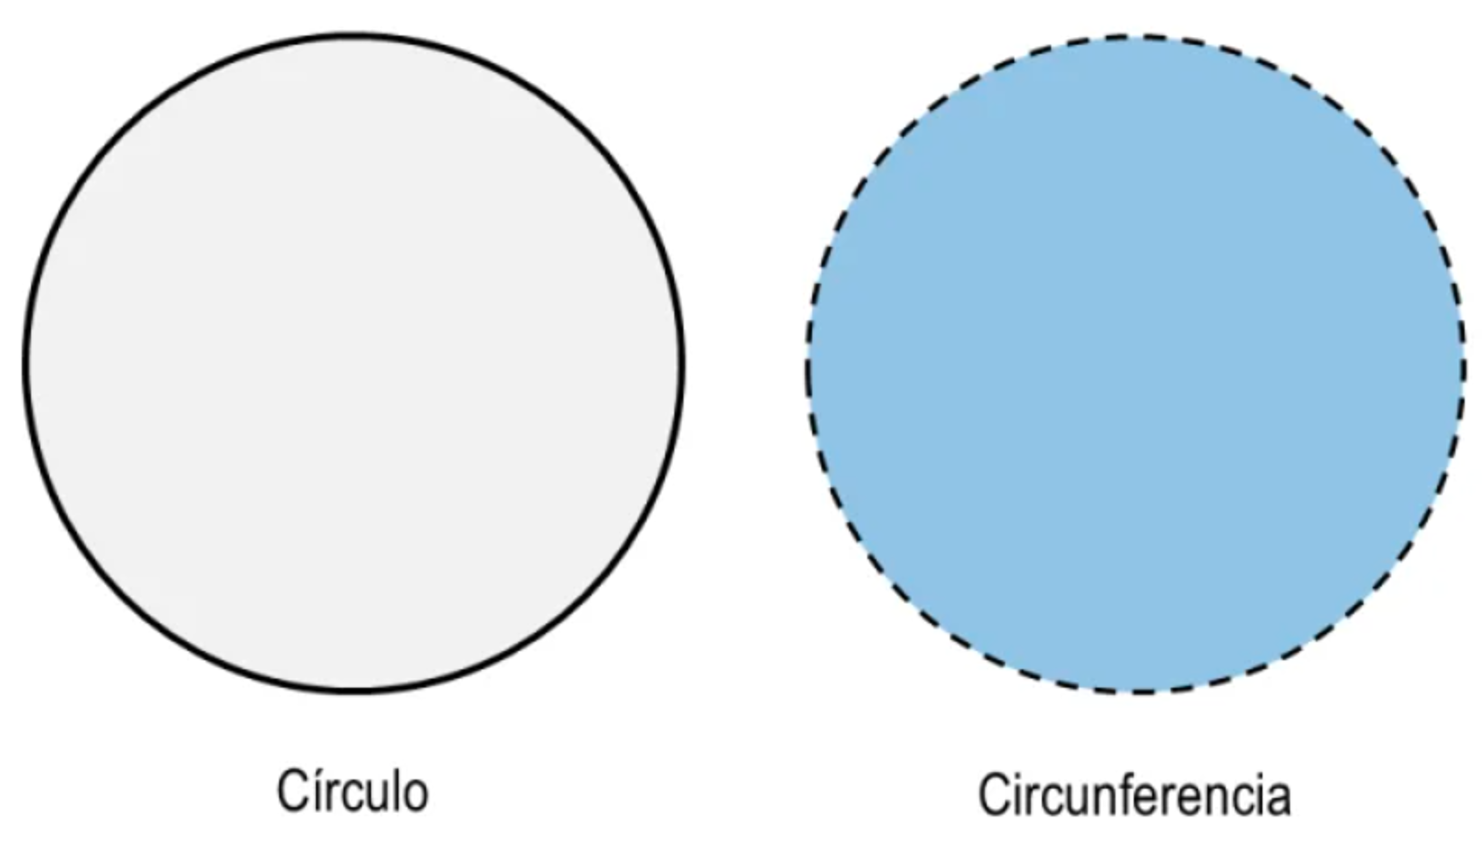
\includegraphics[width = 6cm]{imagen/Circulo, Circunferencia.png}}
\caption{Circulo, Circunferencia}
\label{fig}
\end {figure}

\subsection{Descripción del problema}

Se solicita que una circunferencia con centro en el punto $C$ con coordenadas $(x_{1}, y_{1})$ y radio $r$, se evalué si un punto $T$ con coordenadas $(x_{2}, y_{2})$ esta dentro del área de la circunferencia.

\subsection{Definición de solución}

Primero tenemos que identificar las coordenadas de la circunferencia, que son las coordenadas del centro y así mismo también tenemos que conocer la distancia que hay del centro de la circunferencia hasta cualquier otro punto para así poder saber toda el área que abarca esta circunferencia.

\subsection{Diseño de Solución}
para poder determinar si un punto esta dentro de la circunferencia, primero tenemos que saber el centro de esta circunferencia $(x_{1}, y_{1})$ y a su vez también tenemos que saber la distancia de cualquier otro punto $(x_{2}, y_{2})$ el cual sera nuestro radio que nos ayudara a determinar el área que abarca nuestra circunferencia mediante la siguiente formula:
\begin{equation}
    A = \pi \cdot r^{2}
\end{equation}
Y posteriormente se le solicita al usuario las coordenadas $(x_{3}, y_{3})$ de su punto para determinar si este se encuentra dentro de la circunferencia.
\subsection{Desarrollo de Solución}

\begin{javaCode}
import java.util.Scanner;

public class Circunferencia {
    public static void main(String[] args) {
        Scanner scanner = new Scanner(System.in);
// 
        System.out.println("Ingrese las coordenadas del centro del circulo (x1, y1):");
        double x1 = scanner.nextDouble();
        double y1 = scanner.nextDouble();

        System.out.println("Ingrese las coordenadas de un punto en el circulo (x2, y2):");
        double x2 = scanner.nextDouble();
        double y2 = scanner.nextDouble();

        // Calcula el radio del circulo usando la fórmula de distancia entre dos puntos.
        double radio = Math.sqrt(Math.pow(x2 - x1, 2) + Math.pow(y2 - y1, 2));

        System.out.println("El área del círculo es: " + calcularArea(radio));

        System.out.println("Ingrese las coordenadas de un punto para verificar si esta dentro del círculo (x3, y3):");
        double x3 = scanner.nextDouble();
        double y3 = scanner.nextDouble();

        // Verifica si el punto (x3, y3) está dentro del círculo.
        boolean estaDentro = Math.pow(x3 - x1, 2) + Math.pow(y3 - y1, 2) <= Math.pow(radio, 2);

        if (estaDentro) {
            System.out.println("El punto está dentro del círculo.");
        } else {
            System.out.println("El punto está fuera del círculo.");
        }
    }

    public static double calcularArea(double radio) {
        return Math.PI * Math.pow(radio, 2);
    }
}
\end{javaCode}

\subsection{Depuración y pruebas}

\begin{table}[h]
\centering
\begin{tabular}{|c|c|c|c|c|}
  \hline
  Corrida & X1,Y1 & X2,Y2 & X3,Y3 & ¿El punto está dentro del círculo? \\
  \hline
  1 & 0,0 & 5,5 & 2,3 & SI \\
  \hline
  2 & 9,7 & 3,1 & 8,4 & SI \\
  \hline
  3 & 12,15 & 20,15 & 24,30 & NO \\
  \hline
\end{tabular}
\end{table}

\begin {figure}[h!]
\centerline{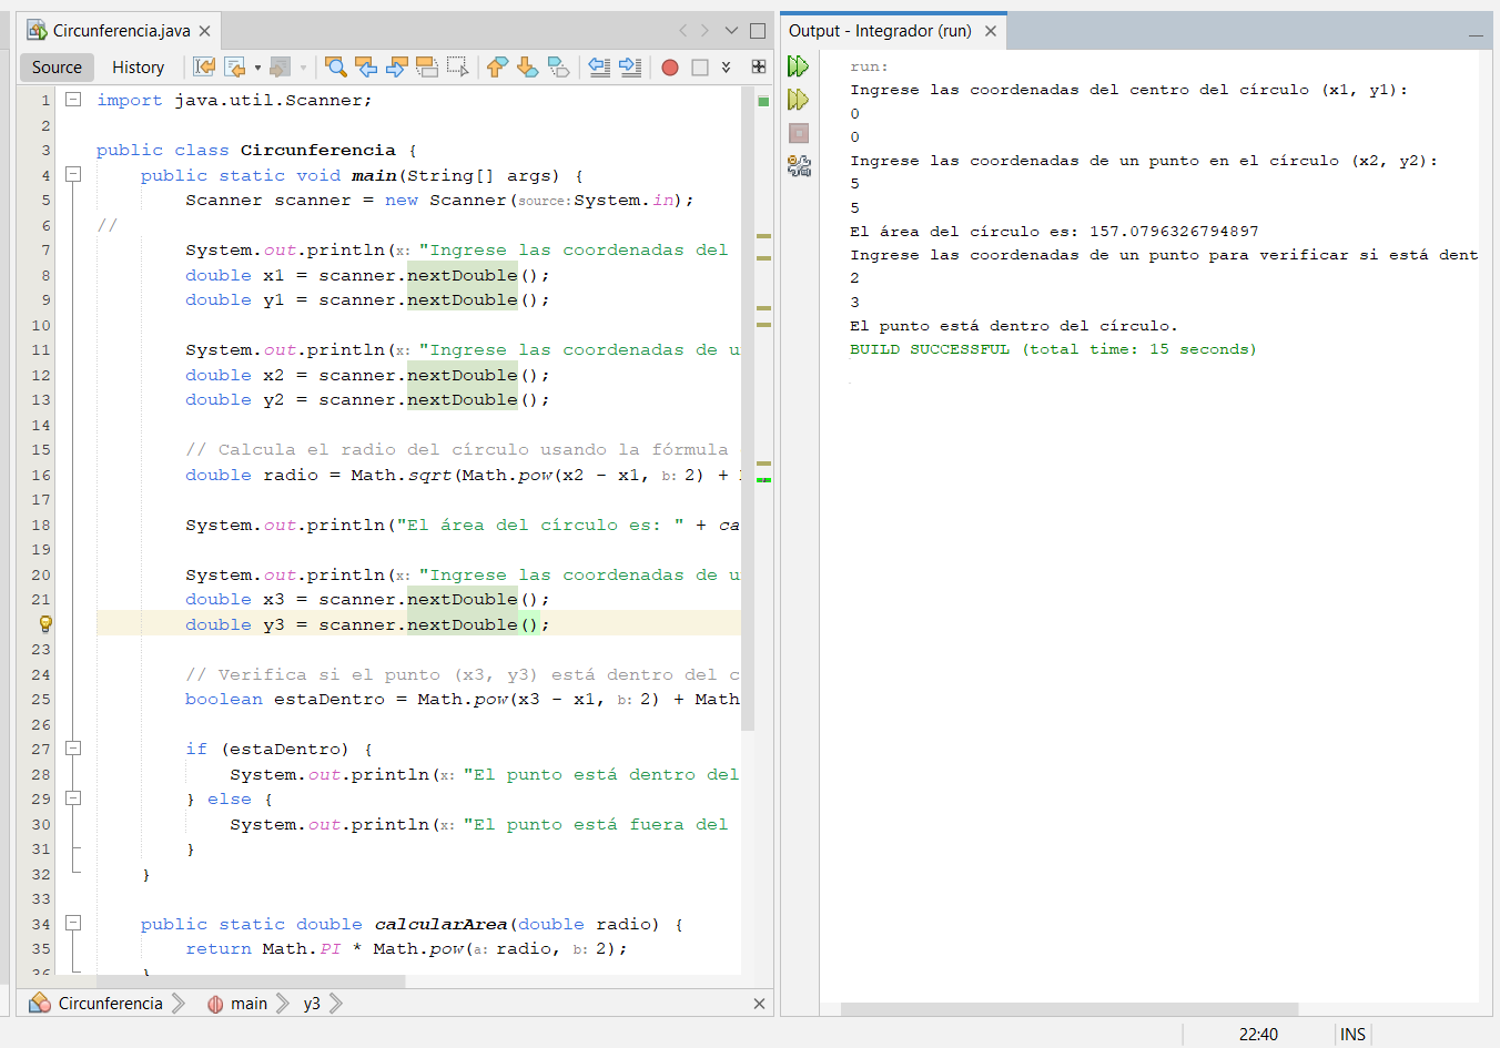
\includegraphics[width = 8cm]{imagen/Corrida1_circunferencia.png}}
\caption{Corrida 1}
\label{fig}
\end {figure}

\begin {figure}[h!]
\centerline{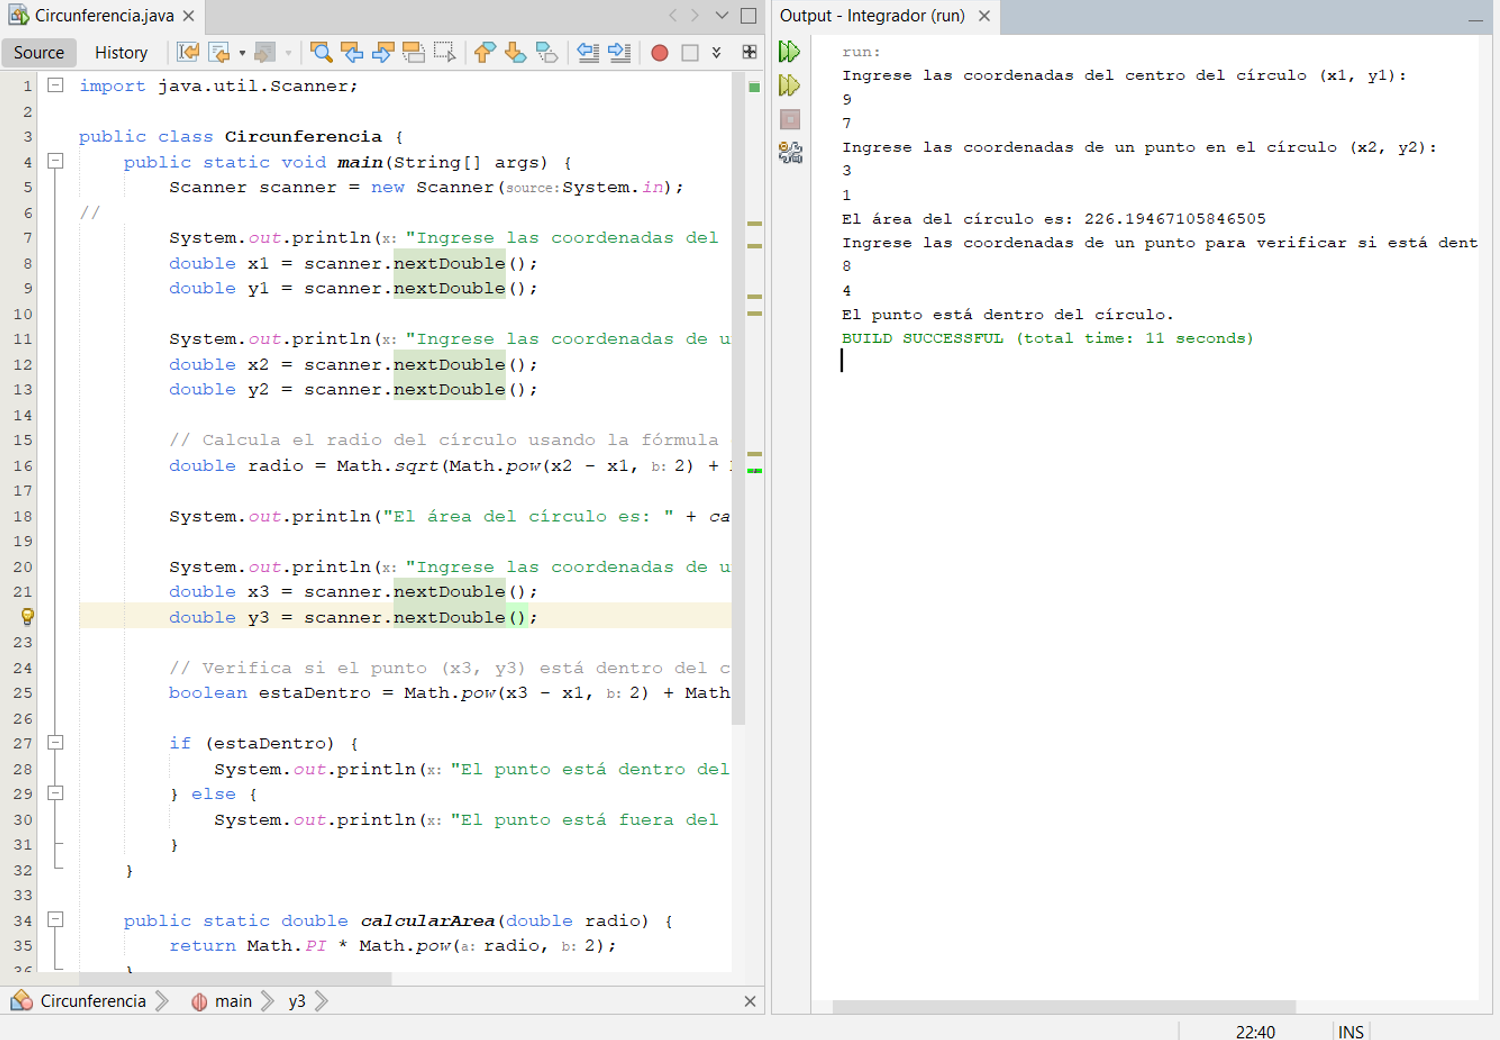
\includegraphics[width = 8cm]{imagen/Corrida2_circunferencia.png}}
\caption{Corrida 2}
\label{fig}
\end {figure}

\begin {figure}[h!]
\centerline{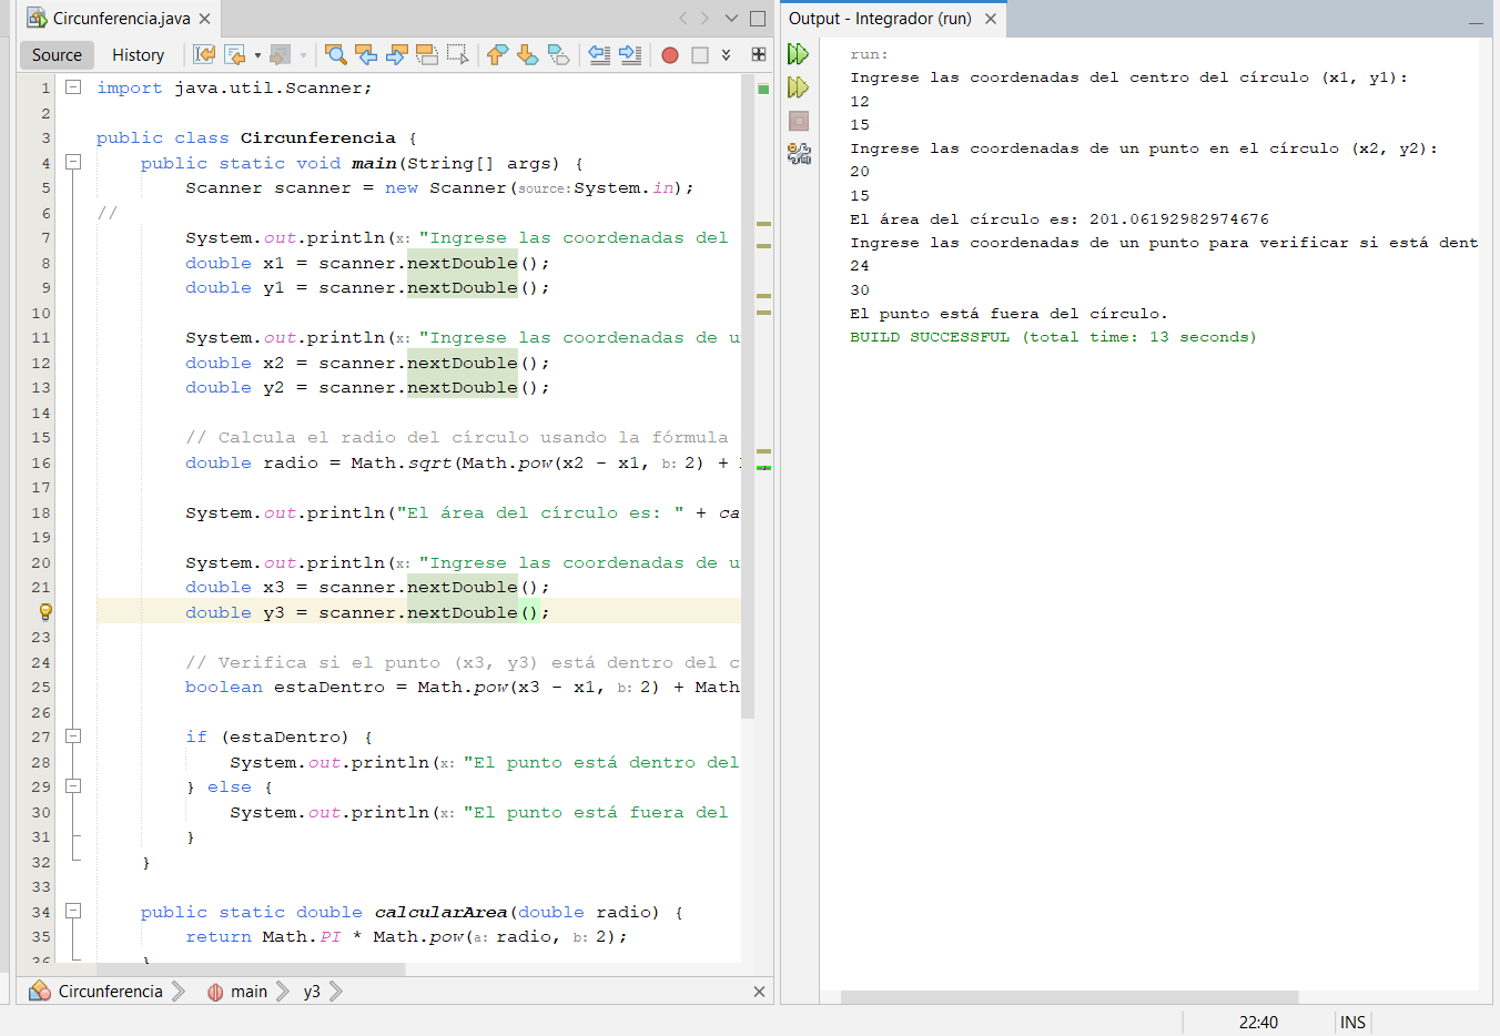
\includegraphics[width = 8cm]{imagen/Corrida3_circunferencia.png}}
\caption{Corrida 3}
\label{fig}
\end {figure}

\section{Sistema Decimal a Sistema Binario}

\subsection{Descripción del problema}
Se solicita que los números decimales se conviertan a números binarios como en positivos y negativos 
\begin {figure}[h!]
\centerline{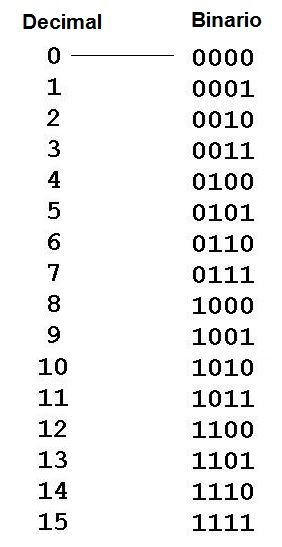
\includegraphics[width = 4cm]{imagen/numeros-binarios.jpg}}
\caption{Binario a decimal.}
\label{fig}
\end {figure}

\subsection{Definición de solución}
Primero se identifican si el número decimal es un entero positivo o negativo, también se le implementara el complemento a dos la cual se ocupa cuando un numero decimal es negativo.
\subsection{Diseño de Solución}
Se solicita un numero decimal, ya sea positivo o negativo, este  sera convertido a numero binario en el cual, se dividirá entre 2 y el resultado también sera divido en 2 hasta que ya no se pueda dividir mas; si el numero decimal es negativo, al convertirlo en binario se hará el mismo procedimiento pero se le impondrá el complemento a dos, en donde se invertirán los bits y se le sumara 1 dándonos hacia el numero binario negativo 
\subsection{Desarrollo de Solución}
\begin{javaCode}
    Scanner scanner = new Scanner(System.in);

        System.out.print("Ingresa un número decimal: ");
        int numeroDecimal = scanner.nextInt();

        String numeroBinario = convertirABinario(numeroDecimal);

        System.out.println("El número binario equivalente es: " + numeroBinario);
    }

    private static String convertirABinario(int numeroDecimal) {
        StringBuilder binario = new StringBuilder();

        if (numeroDecimal == 0) {
            return "0";
        }

        boolean esNegativo = false;
        if (numeroDecimal < 0) {
            esNegativo = true;
            numeroDecimal = -numeroDecimal;
        }

        // Convertir el número decimal a binario
        while (numeroDecimal > 0) {
            int residuo = numeroDecimal % 2;
            binario.insert(0, residuo);
            numeroDecimal /= 2;
        }

        // Calcular el complemento a dos si el número es negativo
        if (esNegativo) {
            // Invertir los bits
            for (int i = 0; i < binario.length(); i++) {
                char bit = binario.charAt(i);
                binario.setCharAt(i, (bit == '0') ? '1' : '0');
            }
            
            // Sumar 1 al complemento invertido
            int carry = 1;
            for (int i = binario.length() - 1; i >= 0; i--) {
                int bit = (binario.charAt(i) - '0') + carry;
                binario.setCharAt(i, (char) (bit % 2 + '0'));
                carry = bit / 2;
            }
        }

        return binario.toString();
    }
}
\end{javaCode}

\subsection{Depuración y pruebas}
\begin{tabular}{|c|c|c|c|}
  \hline
  NumCorrida &Decimal & Binario & C2  \\
  \hline
  1 & 5 & 101 & 1011 \\
  \hline
  2 & 20 & 10100 &  11101100 \\
  \hline
  3 & 60 & 111100 & 11000100\\
  \hline
  
\end{tabular}


\section{Conversión de numero Binario a Decimal}

\subsection{Descripción del problema}
Este programa tiene como objetivo dado un numero binario de n bits regresar su equivalente en decimal.

\begin {figure}[h!]
\centerline{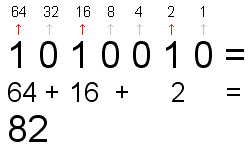
\includegraphics[width = 4cm]{Latex-imágenes/binario.png}}
\caption{Binario a decimal.}
\label{fig}
\end {figure}


\subsection{Definición  de solución}
Para poder hacer la conversión es necesario ingresar un numero binario. Basta con numerar los dígitos de derecha a izquierda comenzando desde cero, a cada número se le asigna la correspondiente potencia base 2 y al final se suman las potencias\cite{articuloBinario} 

\begin {figure}[h!]
\centerline{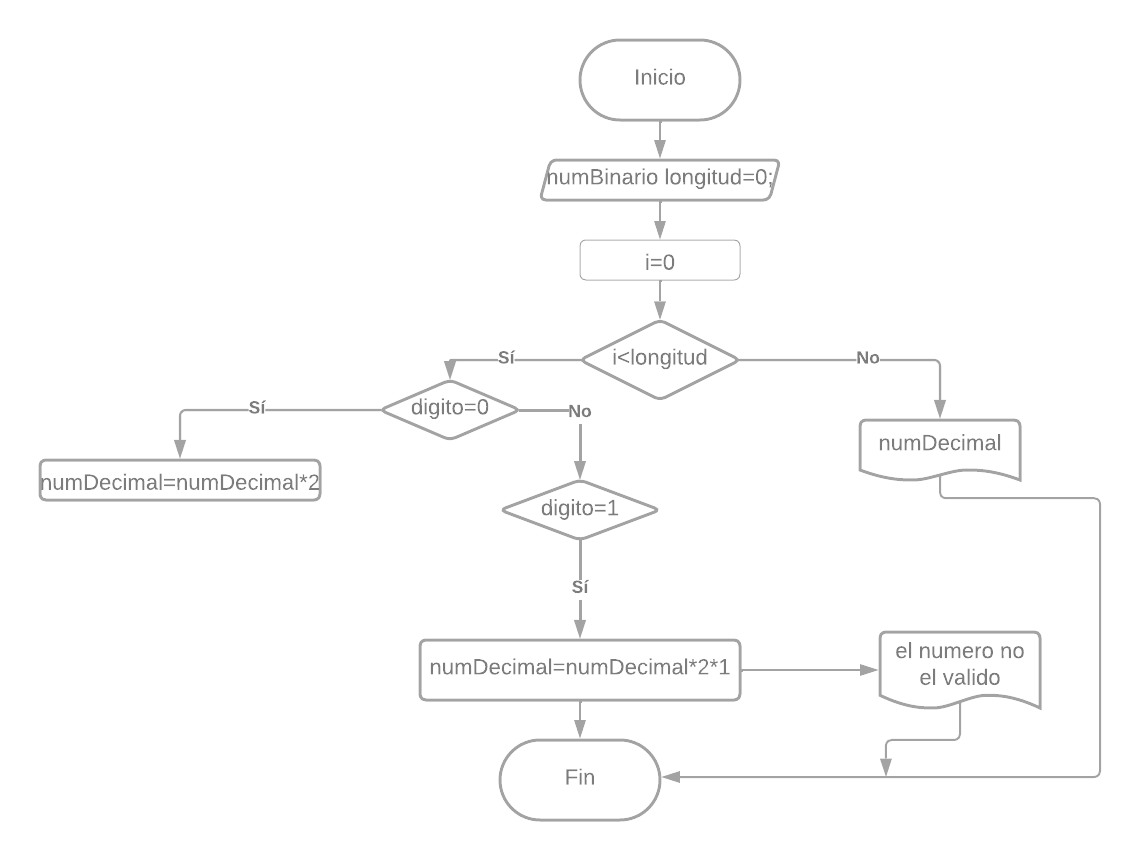
\includegraphics[width = 6cm]{Latex-imágenes/Diagramaejercicio5.png}}
\caption{Binario a decimal.}
\label{fig}
\end {figure}



\subsection{Diseño de Solución}

\begin{enumerate}
  \item El programa comienza pidiendo que se ingrese un numero binario
  \item luego el programa calcula la longitud del numero binario
  \item Se inicia un bucle for que recorre cada dígito del número binario
  \item En cada iteración del bucle, se obtiene el dígito actual utilizando el método charAt(i) y se almacena en la variable digito
  \item Se verifica si el dígito es '0'. Si es así, se multiplica numeroDecimal por 2 sin agregar ningún valor adicional
  \item Si el dígito es '1', se multiplica numeroDecimal por 2 y se le suma 1
  \item Si el dígito no es ni '0' ni '1', se muestra en la consola el mensaje "El numero binario ingresado no es valido"
  \item Después de recorrer todos los dígitos del número binario, se muestra en la consola el resultado de la conversión
  
\end{enumerate}


% En este apartado va el codigo del problea
\subsection{Desarrollo de Solución}
El diseño del programa sigue la estructura y se implementa la .
\begin{javaCode}
int longitud = numeroBinario.length();
        int numeroDecimal = 0;
        for (int i = 0; i < longitud; i++) {
            char digito = numeroBinario.charAt(i);
            //Verificar si es 0 o 1
            if (digito == '0') {
                numeroDecimal = numeroDecimal * 2;
            } else if (digito == '1') {
                numeroDecimal = numeroDecimal * 2 + 1;
            } else {
                System.out.println("El numero binario ingresado no es valido");
                return;
            }
        }
        System.out.println("El numero decimal equivalente es:" + numeroDecimal);
    }
}
\end{javaCode}


%En este apartado va la corrida del ejercicio
\subsection{Depuración y pruebas}
 \begin{tabular}{|c|c|c|}
  \hline
  numCorrida & binario & conversión \\
  \hline
  1 & 101& 5 \\
  \hline
  2 & 0111 & 7 \\
  \hline
  3 & d24 & valor no valido \\
  \hline
\end{tabular}



\section{Conversión de numero Binario a Decimal}

\subsection{Descripción del problema}

Dada una tabla de verdad de n bits generar la expresión booleana que genere de manera fidedigna las salidas de esta tabla. 

\subsection{Definición  de solución}

La solución a este problema implica identificar las operaciones lógicas (como AND, OR, NOT,) y las combinaciones adecuadas de las variables de entrada que permitan reproducir los resultados de la tabla de verdad en todas las combinaciones posibles de los valores de entrada.

\begin {figure}[h!]
\centerline{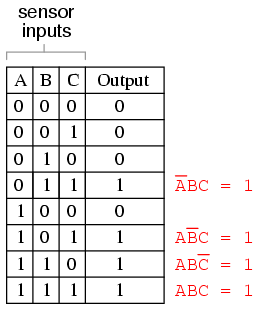
\includegraphics[width = 4cm]{Latex-imágenes/booleanas.png}}
\caption{Binario a decimal.}
\label{fig}
\end {figure}

\subsection{Diseño de Solución}

Para poder codificar la  tabla de verdad  con n bits y la expresión booleana :

\begin{enumerate}
  \item Se crea un conjunto para almacenar las filas que el usuario desea cambiar.
  \item Se solicita al usuario el número de bits.
  \item Se inicia un bucle for que se imprimen los encabezados de las variables (A, B, C, etc.).
  \item Se imprime una fila de la tabla de verdad original y  el resultado, que es siempre 0 en la tabla original.
  \item  Se utiliza while para Bucle para Cambiar Bits y Se lee la fila que el usuario desea cambiar.
   Si el usuario ingresa 0, se sale del bucle.
  \item Se valida que la fila esté en el rango válido. Se vuelve al inicio del bucle si la fila no es válida.
  \item Se imprimen las expresiones booleanas asociadas a las filas modificadas. Se imprime la expresión booleana final.
  \item Se imprime cada bit de la fila en formato binario. Se imprime el resultado (1 o 0) de acuerdo a las filas cambiadas.
  \item Se genera la expresión booleana para una fila específica.
  \item Se genera la expresión booleana final concatenando las expresiones de las filas modificadas.
  
\end{enumerate}

\subsection{Desarrollo de Solución}


\begin{javaCode}
import java.util.Scanner;

public class Ejercicio_6_basico {
    public static void main(String[] args) {
        Scanner scanner = new Scanner(System.in);
        
        System.out.print("Ingrese el número de bits para la Tabla de Verdad: ");
        int numBits = scanner.nextInt();
        
        // Imprime encabezados de las variables
        for (int i = 0; i < numBits; i++) {
            System.out.print((char) ('A' + i) + "\t");
        }
        System.out.println("Resultado");
        
        // Inicializa la tabla de verdad con todos los resultados en 0
        int[] tablaVerdad = new int[(int) Math.pow(2, numBits)];
        
        // Imprime tabla de verdad original
        imprimirTabla(tablaVerdad, numBits);
        
        // Cambia las filas
        while (true) {
            System.out.print("Ingrese el número de la fila que desea cambiar a 1 (1-" + (int) Math.pow(2, numBits) + ") o ingrese 0 para finalizar: ");
            int fila = scanner.nextInt();
            
            if (fila == 0) {
                break;
            }
            
            if (fila < 1 || fila > Math.pow(2, numBits)) {
                System.out.println("Número de fila inválido. Debe estar entre 1 y " + (int) Math.pow(2, numBits) + ".");
                continue;
            }
            
            tablaVerdad[fila - 1] = 1;
            
            imprimirTabla(tablaVerdad, numBits);
        }
    }

    private static void imprimirTabla(int[] tablaVerdad, int numBits) {
        System.out.println("Tabla de verdad actualizada:");
        for (int i = 0; i < tablaVerdad.length; i++) {
            imprimirFilaTabla(i, numBits);
            System.out.println(tablaVerdad[i]);
        }
    }

    private static void imprimirFilaTabla(int valor, int numBits) {
        for (int j = numBits - 1; j >= 0; j--) {
            System.out.print(((valor >> j) & 1) + "\t");
        }
    }
}
\end{javaCode}

\subsection{Depuración y pruebas}

\begin {figure}[h!]
\centerline{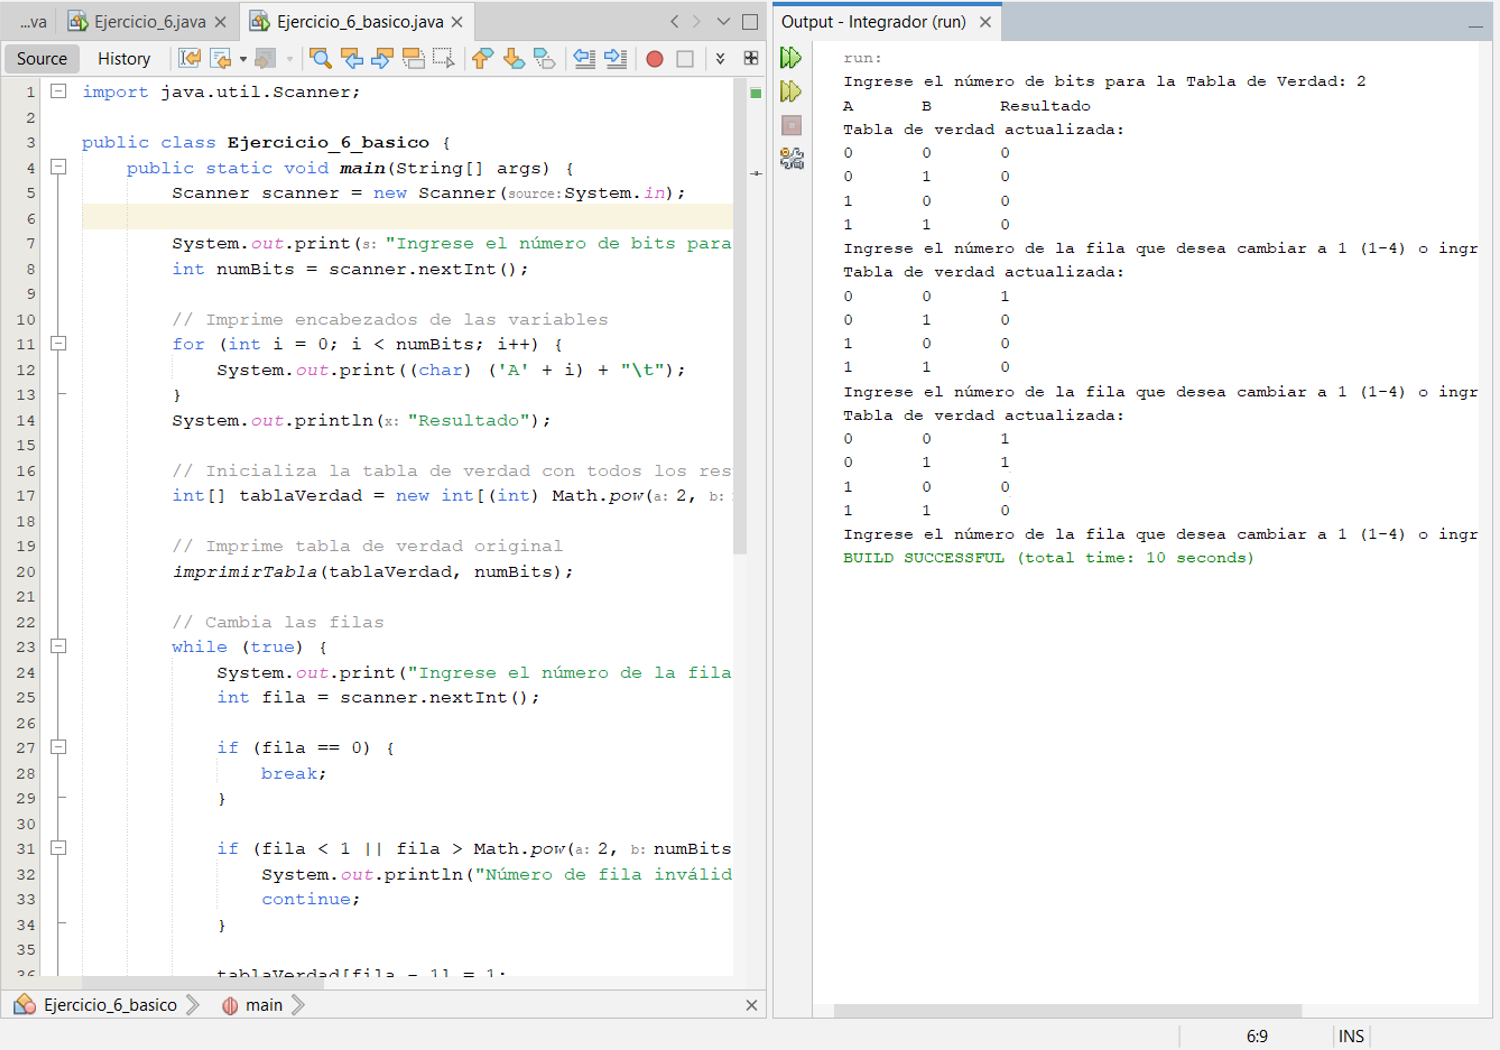
\includegraphics[width = 9.5cm]{Latex-imágenes/tabla de verdad de 2 datos.png}}
\caption{Corrida 3}
\label{fig}
\end {figure}

\begin {figure}[h!]
\centerline{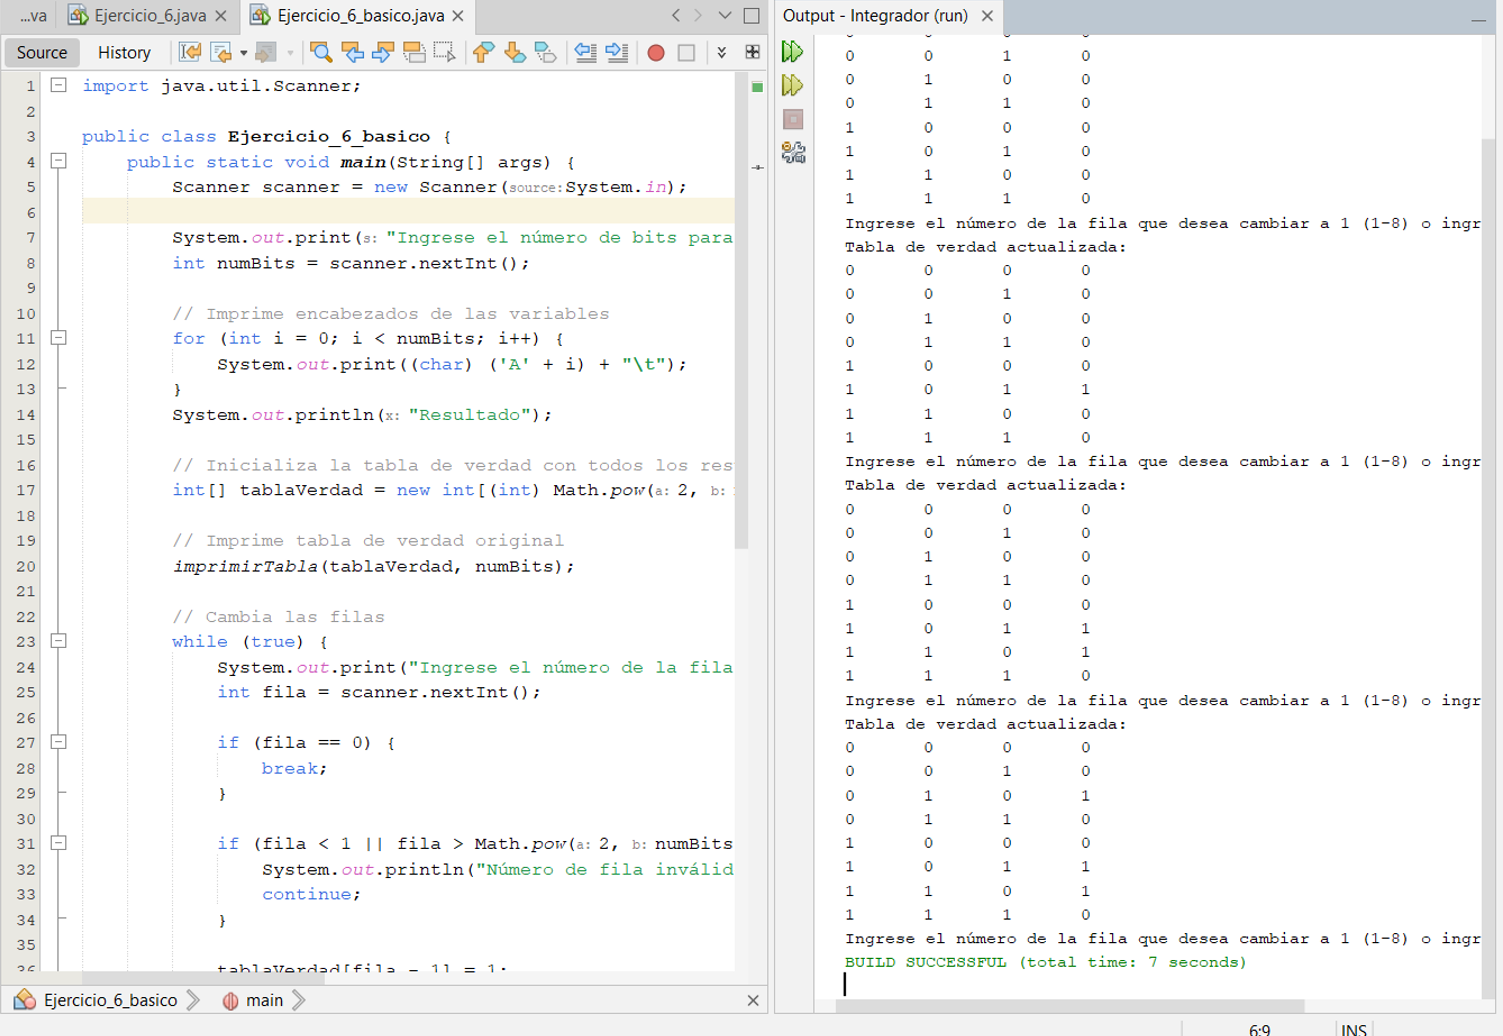
\includegraphics[width = 9.5cm]{Latex-imágenes/tabla de verdad de 3 datos.png}}
\caption{Corrida 3}
\label{fig}
\end {figure}


%en esta session va la conclusion 
\subsection{Conclusión}

En este proyecto concluimos diversos problemas  de principio a fin.  A lo largo del proceso, nos enfrentamos a desafíos matemáticos y algorítmicos los cuales, con dedicación y colaboración, logramos resolver de manera satisfactoria.

Este proyecto no solo puso a prueba nuestras habilidades técnicas en el ámbito de nuestras materias, sino que también ayudo nuestra capacidad para abordar problemas matemáticos desde una perspectiva práctica. La intersección entre las matemáticas y la programación nos permitió no solo comprender la teoría, sino aplicar estos conocimientos de manera efectiva para encontrar soluciones correctas.

Es importante recalcar que como integrantes aprendimos a trabajar mejor en equipo, cada uno propuso sus ideas y tomamos en cuenta cada una de estas, había ciertos bloques de temas en los cuales nos costa baba mas lo habitual anteriormente. 

Al finalizar este proyecto, no solo hemos alcanzado nuestras metas, sino que también hemos adquirido una comprensión más profunda. Este conocimiento no solo es valioso en términos académicos, sino que también se traduce en habilidades prácticas que pueden aplicarse en diversos contextos profesionales.
Creemos que estos proyectos ayudan a consolidar a el alumno como un estudiante competente para que pueda estar futuros proyectos a nivel profesional, cada proyecto brinda la experiencia lo que hace que seas mejor en cada aspecto que trabajes.

\subsection{Agradecimientos}
Gracias  Goggle, poe y chatGPT y mas importante al bicho por motivarme  a seguir adelante

%librero de reporte integrador
\begin{thebibliography}{00}
  \bibitem{articuloRecta}
  Khan Academy, October 20, 2023, Tangent lines and rates of change,
  https://www.khanacademy.org/math/calculus-all-old/taking-derivatives-calc/using-the-formal-definition-of-derivative-calc/a/tangent-lines-and-rates-of-change


    \bibitem{articuloEcuación}
    Comprender la fórmula de la cuadrática (artículo) | Khan Academy. (s. f.). Khan Academy. https://es.khanacademy.org/math/algebra-home/alg-quadratics/alg-solving-quadratics-using-the-quadratic-formula/a/quadratic-formula-explained-article


    \bibitem{articulocirCunferencia}
    Revisión de ecuación del círculo (artículo) | Khan Academy. (s. f.). Khan Academy. https://es.khanacademy.org/math/eb-3-semestre-bachillerato-nme/x4b655b3cb9bfe4eb:ecuacion-de-la-circunferencia/x4b655b3cb9bfe4eb:ecuacion-general-de-la-circunferencia/a/circle-equation-review

    \bibitem{articuloDecimalBinmario}
    Sistemas binarios y decimales. (s. f.). EDteam - En español nadie te explica mejor. https://ed.team/blog/sistemas-binarios-y-decimales

    \bibitem{articuloBinario}
    Sistemas binarios y decimales. (s. f.). EDteam - En español nadie te explica mejor. https://ed.team/blog/sistemas-binarios-y-decimales#
    
\end{thebibliography}

\subsection{Biografías}

\textbf{Lozano Camargo Diego} \\
Es estudiante del Instituto Tecnológico Superior del Occidente del Estado de Hidalgo, que actualmente cursa el primer semestre en la carrera de Ingeniería en Tecnologías de la Información y Comunicaciones(TICs). Nació en Actopan Hidalgo el 19 de Marzo del 2005 y actualmente tiene 18 años, le gusta jugar fútbol, ver series en su tiempo libre así como jugar videojuegos y salir con sus amigos. \\
\href{https://github.com/diego2334577}{GitHub de Diego Lozano Camargo}

\textbf{Reyes Garcia Azucena} \\
Estudiante actual del Instituto Tecnológico Superior del Occidente del Estado de Hidalgo, estudia el primer semestre en la carrera de Ingeniería  en Tecnologías de la Información y la Comunicaciones (TIC's), Nació el 30 de septiembre del 2005 en la localidad de Panuaya  Municipio de Tezontepec de Aldama, Estado de Hidalgo. Estudio el preescolar, primaria y secundaria en la localidad donde actualmente se encuentra viviendo, San Gabriel, posteriormente estudio la preparatoria en el Colegio de Bachilleres (Plantel Atengo) donde fue reconocida por el proyecto ACMAS el cual fue un impacto a nivel subsistema ya que 50 planteles fueron beneficiados. \\
\href{https://github.com/AzucenaReyesGarcia}{GitHub de Azucena Reyes Garcia}\\

\textbf{Guerrero Hernandez Xavier Amed} \\
Un joven estudiante que nació el 17 de febrero de 2005 en Tula de Allende Hidalgo, estudia el primer semestre de (TICs) en Instituto Tecnológico Superior del Occidente del Estado de Hidalgo paso su kinder y primaria en su pueblo Atitalaquia, para después estudiar la secundaria en un pueblo llamado Cardonal,terminó la prepa en el Colegio de bachilleres de Atotonilco de Tula, fue 3er lugar del Estatal de 100 metros en Pachuca. \\
\href{https://github.com/XavierGuerreroo}{GitHub de Xavier Amed Guerrero Hernandez} \\

\textbf{Lopez Gonzales Daniel} \\
%poner su biografia
Joven estudiante actual del Instituto Tecnológico Superior del Occidente del Estado de Hidalgo, estudia el primer semestre de Ingeniería de Tecnología de la Información y la Comunicaciones (ITICs), nació el 12 de noviembre de 2004 en Chilcuautla, Hidalgo, se localiza en la localidad de Tlacotlapilco, municipio de Chilcuautla, paso el preescolar y primaria en su localidad de Tlacotlapilco, su secundaria lo concluyo en la localidad de Santa Ana Batha, al igual que su preparatoria. \\
\href{https://github.com/LopezDanielgod}{GitHub de Daniel Lopez Gonzalez}\\

\textbf{Murillo Martínez Kleyder} \\
%poner su biografia
Actualmente es estudiante del Instituto Tecnológico Superior del Occidente del Estado de Hidalgo (ITSOEH) en la carrera de Tecnologías de la Información Y la Comunicación (TIC´s). Nació el 10 de mayo del 2005 en Ixmiquilpan HGO. Estudio su primaria y secundaria en Progreso de Obregón Hidalgo que es donde vive actualmente, y su bachillerato lo termino en el municipio del Tinaco, el cual le pertenece a Tezontepec de Aldama.
Sus gustos son: los videojuegos, la musica y programar en Arduino, y actualmente busca reforzar sus conocimientos para así poder saber mas sobre el mundo en el que vivimos.
\href{https://github.com/KleyderMurillo}{GitHub de Kleyder Murillo Martínez}

\end{document}